\section{Numerical Results}
\label{sec:numres} 
All update equations as defined in Section \ref{subsec:timestepeqs} were implemented in Rust. This language was chosen for its C++ like performance while enforcing compile-time memory safety which makes writing fast and safe CEM codes relatively easy. An overview of this implementation can be found in \ref{subsec:code}.

\subsection{Verification and Validation}
\label{subsec:vv}
To verify and validate model results, the case of an infinitely long waveguide with fields propagating in the $\mathrm{TE_{10}}$ mode. This case is chosen as simulated results can easily be compared to analytic results.

All verification and validation analyses are performed with $0.1$m stretch of a WR-90, X-band waveguide with a free space-filled, cross section of $a=0.02286$m and $b=0.01016$m \cite{everythingrf}. Said configuration has an analytic $\mathrm{TE_{10}}$ cutoff frequency of as calculated by
\begin{align}
    f_c=\frac{c}{2\pi\sqrt{\epsilon_r\mu_r}}\sqrt{\bigg[\frac{m\pi}{a}\bigg]^2}
    \label{eq:analytic-cutoff}
\end{align}
from \cite{pozar2011microwave}. Using free space dielectric parameters, this geometry has a cutoff frequency of $6.557$GHz for the $\mathrm{TE_{10}}$ mode.

To ensure waves above the cutoff frequency are able to freely propagate, a monochromatic source as defined by (\ref{eq:tapered-sin}) is used with a $10$GHz carrier frequency with a ramp time of $5$ns is used as an $E_y$ driver function. The simulation was carried out using a time step of $\Delta t=1.863$ps over a $25$ns duration with spatial steps as $\Delta x=0.994$mm, $\Delta y=0.923$mm, and $\Delta z=0.990$mm.

A spatial field profile of this system can be found in Fig. \ref{fig:profile} along the $y$ and $x$ centerline planes.

\begin{figure}[h!]  
	\centering
	%the command within the [] sets the width of the figure, stability-condition is the jpg name
	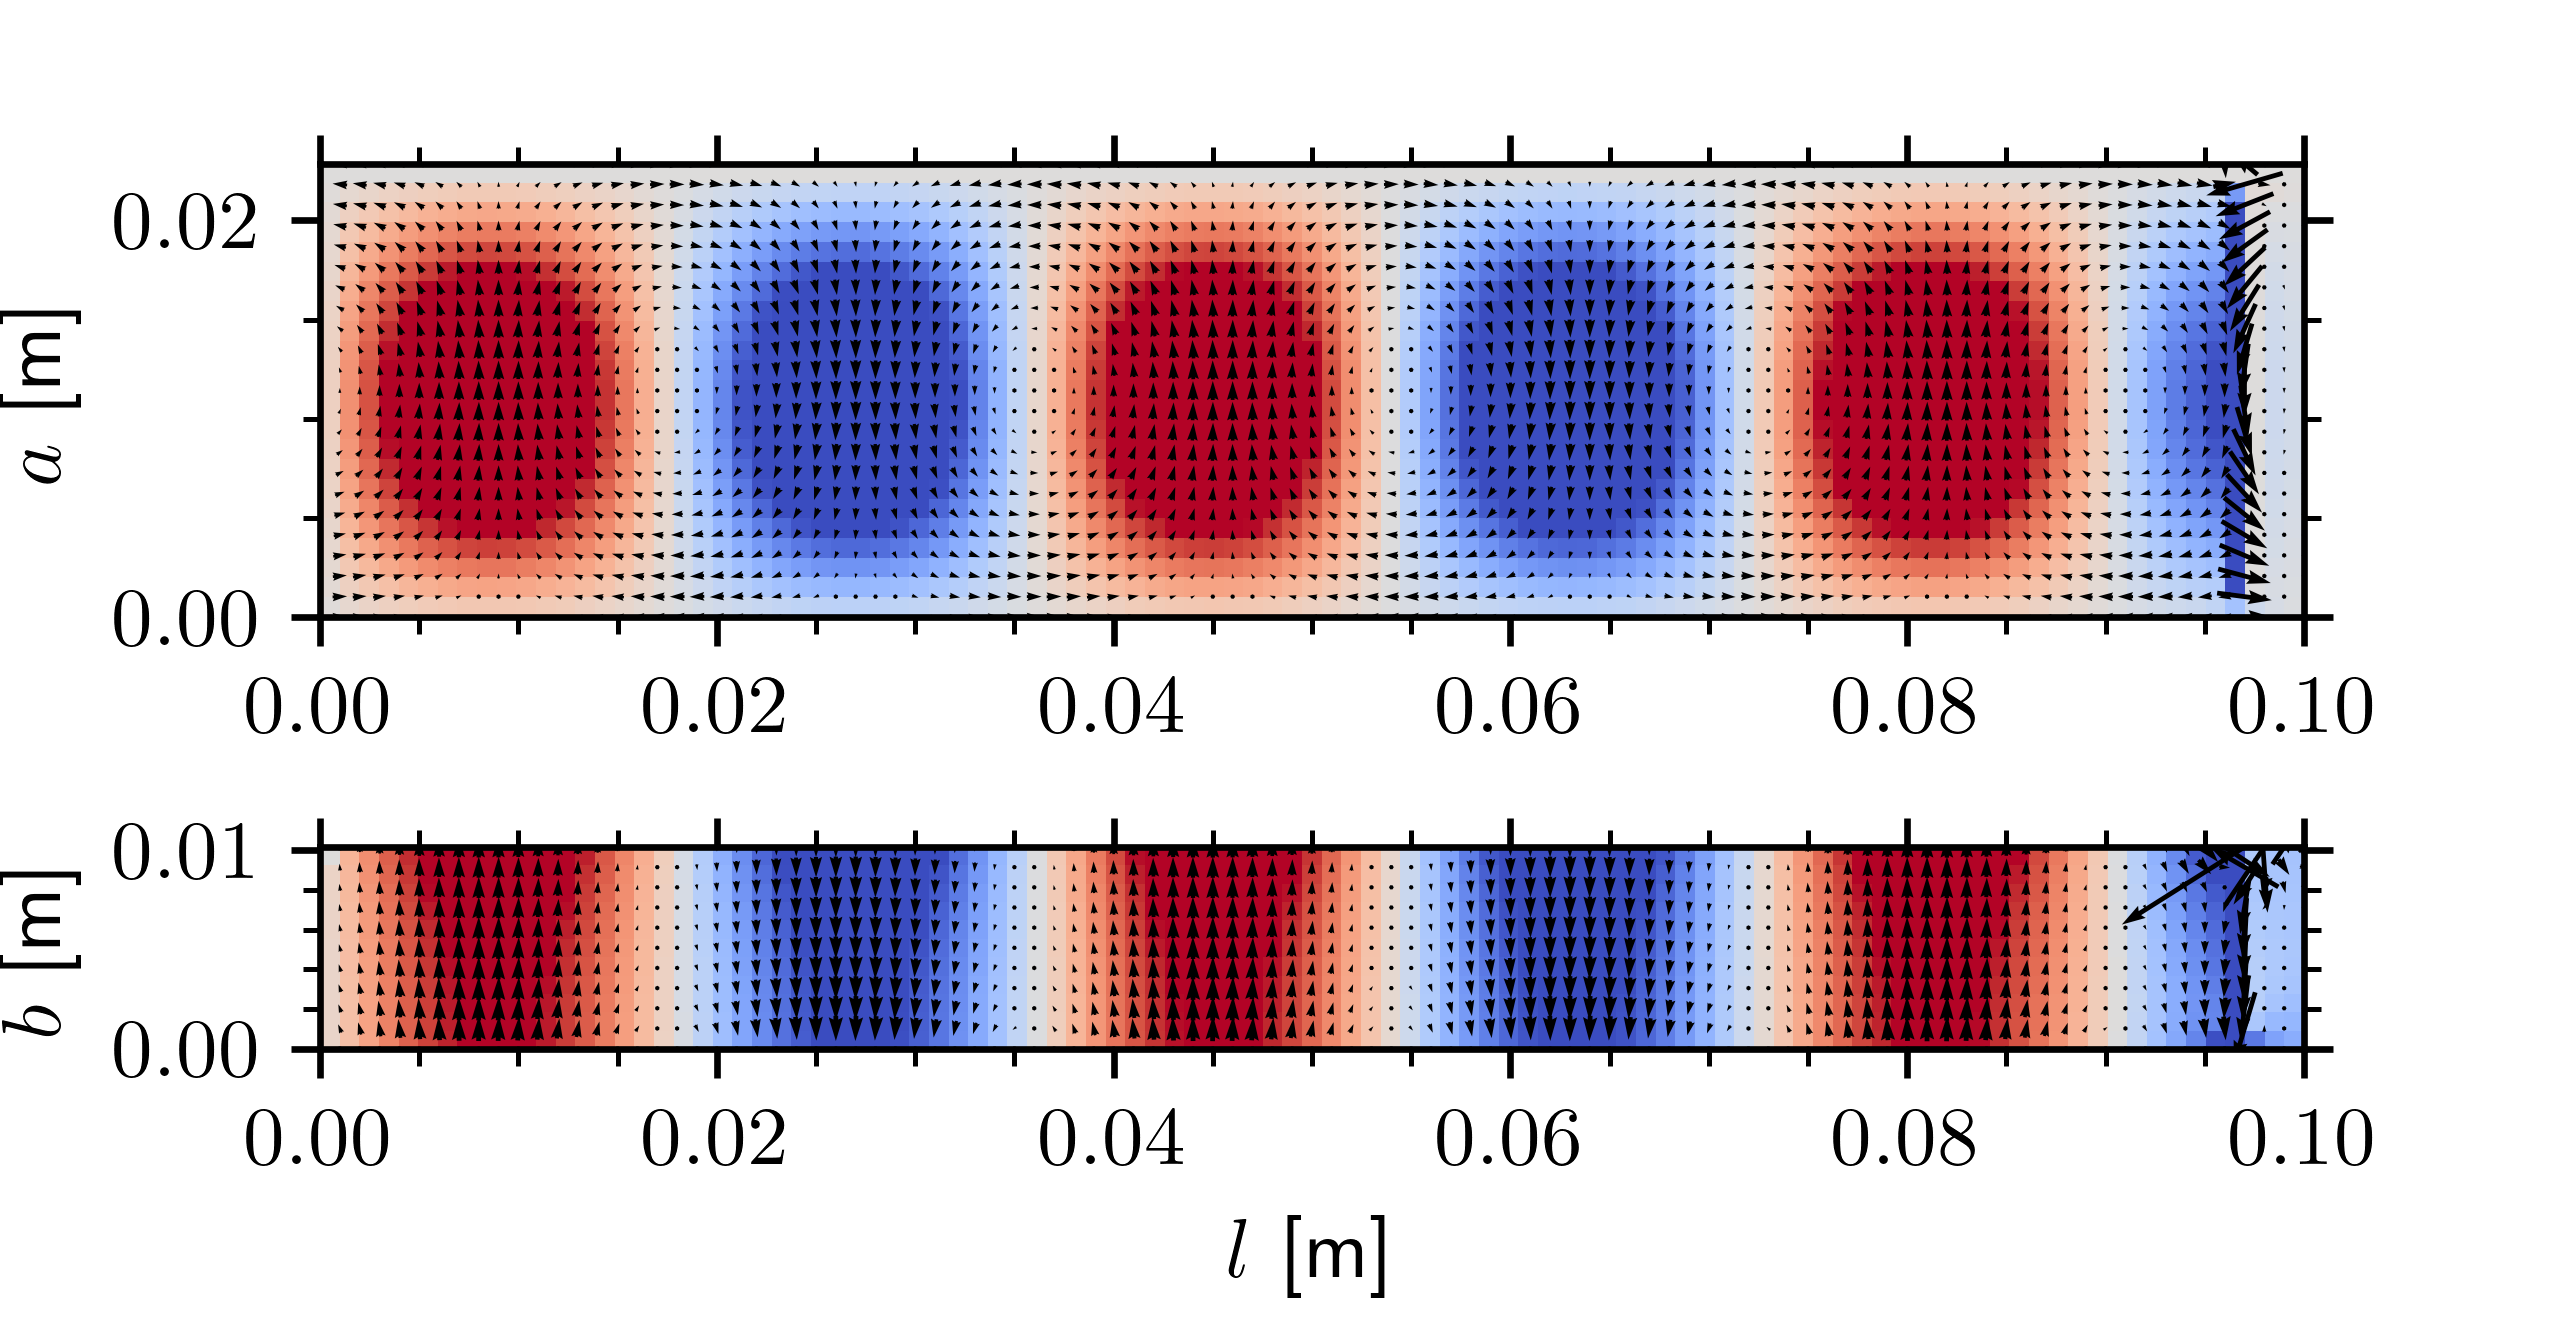
\includegraphics[width=\columnwidth]{labeled-monochromatic-source-profile.png} 
	\caption{Source Profiles at $t=8.191$ns for (a) $E_y$ intensity (colored) with $H_x, H_y$ directions (arrows) along the $y=5.538$mm plane and (b) $H_x$ intensity (colored) with $E_y, E_z$ directions (arrows) along the $x=11.926$mm plane}
	\label{fig:profile}
\end{figure}

Arrows in Fig. \ref{fig:profile} were scaled as to best show direction where as intensity colors were based off of the $E_y$ sinusoidal amplitude. Colors for Fig. \ref{fig:profile} (b) are scaled down by $E_y / \eta_{10}$ as in (\ref{eq:hxfreq}). Field intensity was not explicitly labeled in Fig. \ref{fig:profile} as it cluttered the plots and is not relevant for this analysis. 

From visual inspection, it is quite clear that these field profiles match the theoretical frequency domain profiles as given in (\ref{eq:eyfreq}-\ref{eq:hxfreq}). Additionally, the validity of the TF/SF source and Mur's ABC is apparent from the relatively small fields found in the upper right of Fig. \ref{fig:profile} (a) and (b). The small discrepancy in the upper right corner of \ref{fig:profile} (b) is explained by leakage of the TF/SF source interacting with the PEC corner; both of which are liable for discrepancies as mentioned in \cite{rothlecnotes}.

To ensure the integrity of the wave propagating along the length of the waveguide, frequency spectra are taken of the source total field and transmitted total $E_y$ field as found in Fig. \ref{fig:mono-spectra}. These transmitted and source spectra were taken at two representative voxels at $z=4.950$mm and $z=95.050$mm along the same $x$ and $y$ centerlines of Fig. \ref{fig:profile}. This choice of a centerline is arbitrary; changes in the $x$ position would decrease the relative field intensity due to the sinusoidal profile necessitated by the PEC walls. Data for this plot was obatined by taking a field `snapshot' $2,000$ times over a the span of the $25$ns simulation window with intermediate time spacing between samples of $13.043$ps.
\begin{figure}[h!]  
	\centering
	%the command within the [] sets the width of the figure, stability-condition is the jpg name
	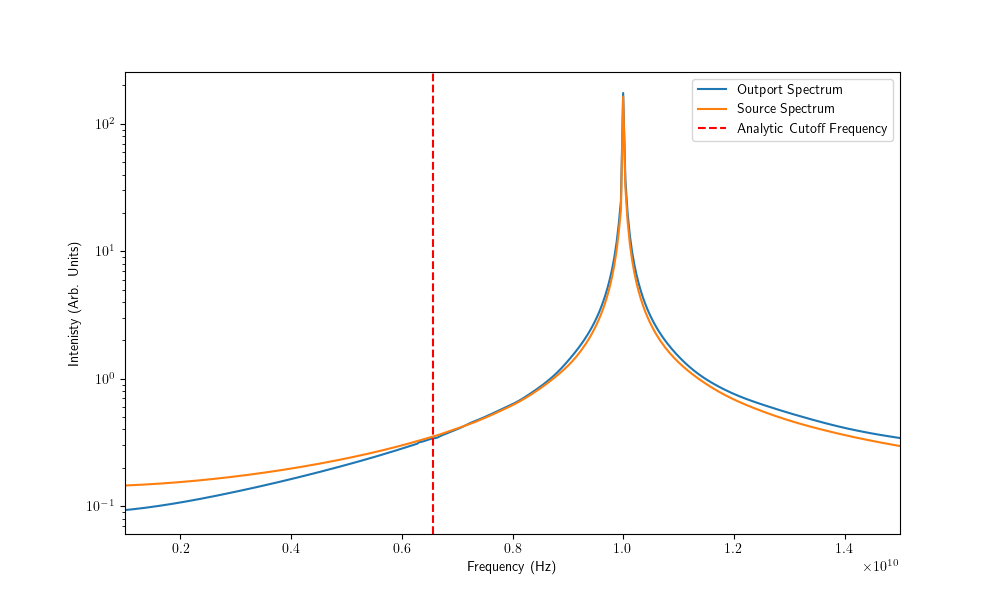
\includegraphics[width=\columnwidth]{monochromatic-source.png} 
	\caption{Transmitted and Source Frequency Spectra with Labeled Cutoff Frequency for $10$GHz Monochromatic Tapered Sine $E_y$ Source}
	\label{fig:mono-spectra}
\end{figure}

Fig. \ref{fig:mono-spectra} clearly shows that all frequencies above the $6.557$GHz cutoff frequency are able to travel along the length of the waveguide with minimal loss. These signals only differ for frequencies below that of the cutoff frequency of which fields are not able to propagate indefinitely.

With frequencies above the cutoff frequency able to freely propagate in the waveguide, it is now important to assess the waveguides performance in attenuating waves below the cutoff frequency. To test this property of our simulated waveguide, a wide-band modulated gaussian pulse as in (\ref{eq:mod-gauss}) is used as a driver signal with a carrier frequency of $10$GHz, ramp time of $0.5$ns and delay time of $3ns$. Frequency spectra at identical locations to that of Fig. \ref{fig:mono-spectra} can be found below in Fig. \ref{fig:wide-spectra}. To facilitate the additional frequency content of the modulated Gaussian, field snapshots were waken at all $13,417$ time steps over the simulation's $25$ns duration.  

\begin{figure}[h!]  
	\centering
	%the command within the [] sets the width of the figure, stability-condition is the jpg name
	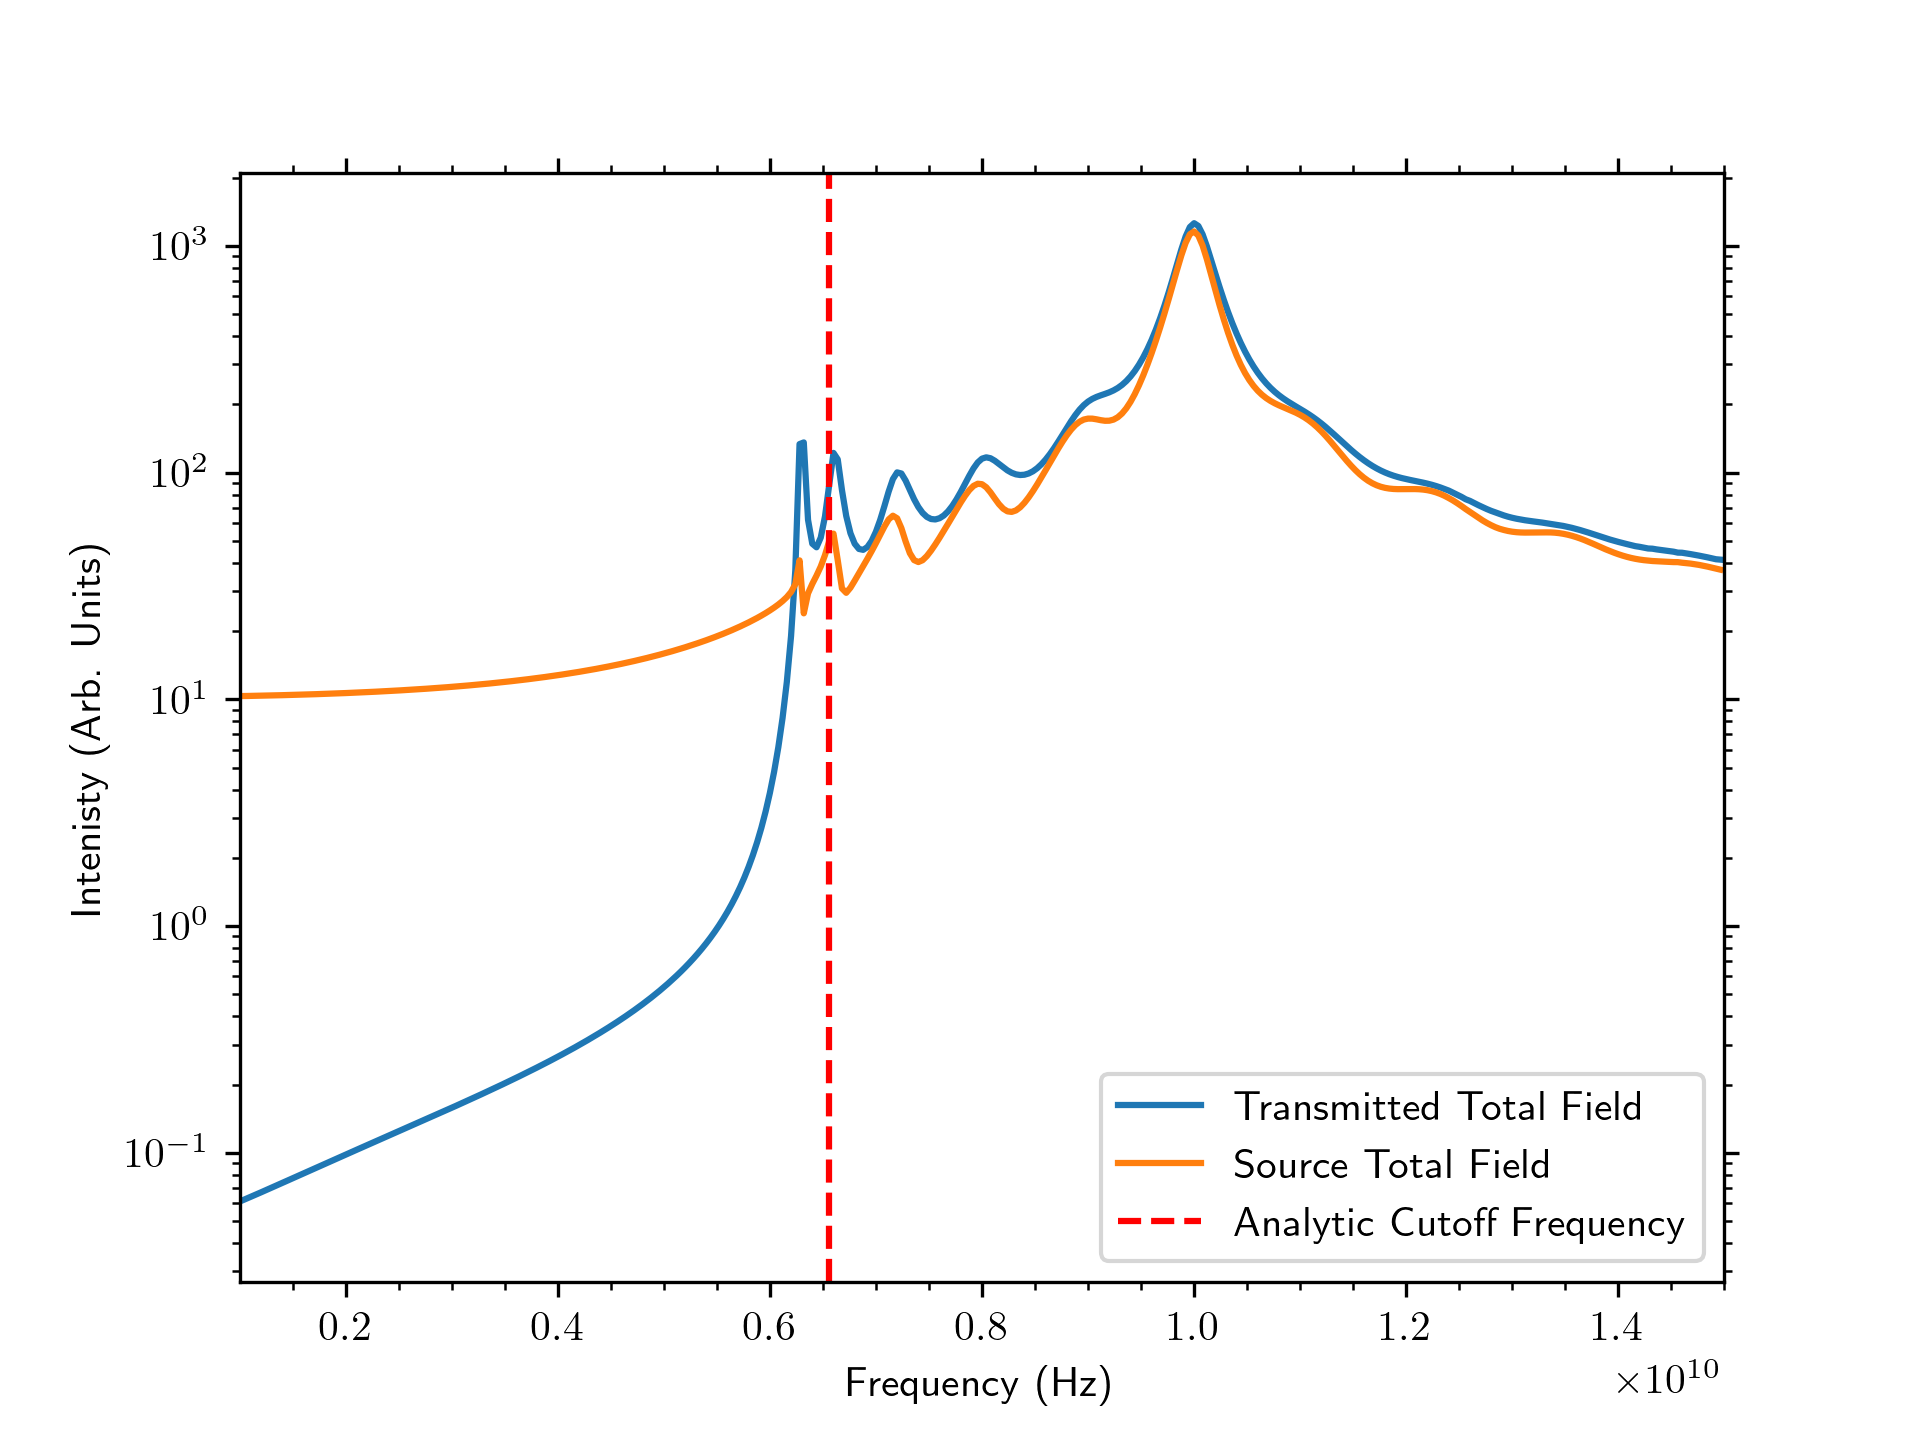
\includegraphics[width=\columnwidth]{wideband-spectrum.png} 
	\caption{Transmitted and Source Frequency Spectra with Labeled Cutoff Frequency for $10$GHz Center Frequency, $0.5$ns Ramp Time, Modulated Gaussian Pulse}
	\label{fig:wide-spectra}
\end{figure}

As shown above in Figure \ref{fig:wide-spectra} the \textit{in silico} waveguide exhibits a cutoff frequency of approximately $6.2$GHz which only differs from the theoretical by $5.444\%$ making this model relatively realistic. Below this cutoff frequency, Fig. \ref{fig:wide-spectra} shows a nearly two order of magnitude reduction in the transmitted while having little overall impact on frequencies above this which is expected.

\subsection{Analysis of Unloaded Quality Factor with Varying Dielectric Loss}
\label{subsec:dielectric-loss}
With the waveguide now successfully validated, the resonator performance can now be assessed using different dielectric materials. More specifically, we aim to compare the performance of a cavity resonator filled with beeswax to that filled with beryllia at a frequency of $10$GHz. Material properties for these materials are obtained from \cite{pozar2011microwave} which are used to derive conductivities for these materials at $25^oC$. For simplicity, the resonator cavity length is reduced from $0.1$m to $0.05$m to reduce the computational domain. An identical wideband carrier signal to that found in Fig \ref{fig:wide-spectra} is used to look for resonances in these materials at and around $10$GHz. For these simulations, the centermost $E_y$ voxel is used as a representative sample of the whole domain. Due to these materials differing relative permittivities, the centermost voxel may exist at slightly different physical locations within the simulation; however, this discrepancy is assumed to be small. results for this comparative study can be found below in Fig. \ref{fig:comp-spectra}.

\begin{figure}[h!]  
	\centering
	%the command within the [] sets the width of the figure, stability-condition is the jpg name
	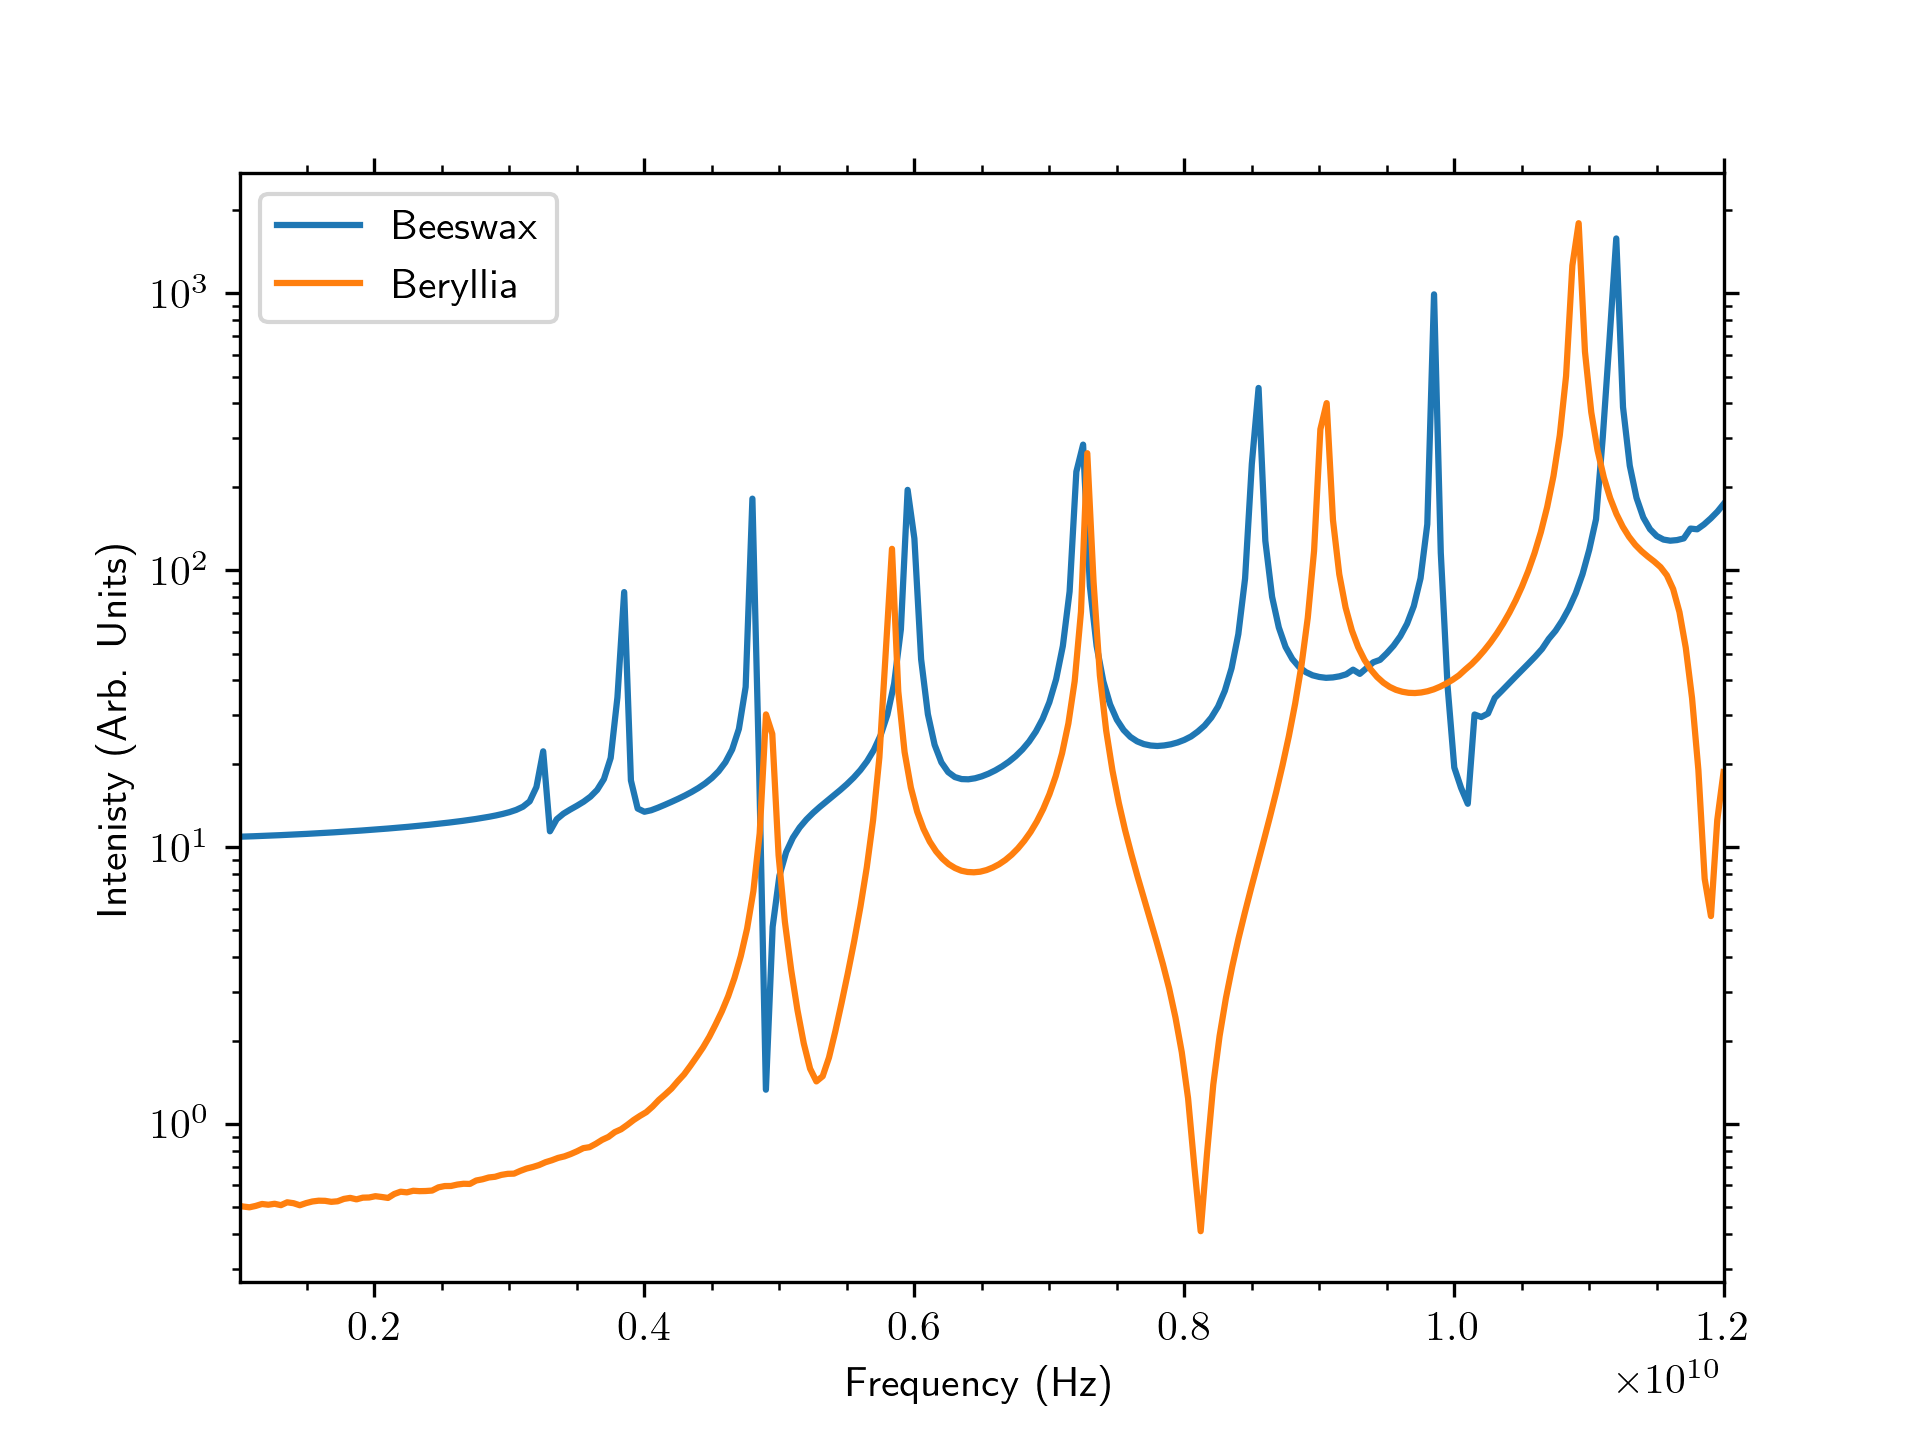
\includegraphics[width=\columnwidth]{comp.png} 
	\caption{Centermost Voxel Frequency Spectra for Beeswax and Beryllia for $10$GHz Center Frequency, $0.5$ns Ramp Time, Modulated Gaussian Pulse}
	\label{fig:comp-spectra}
\end{figure}

These two materials exhibit far more complex interactions than that of free space with numerous resonances exited in both materials. With its lower loss tangent of $\tan\delta=0.0003$ and higher unloaded dielectric quality factor $Q=3333.3$, beryllia resonates several times more than beeswax with a loss tangent of $\tan\delta=0.005$ and $Q=200$ at $10$GHz. Interestingly the beeswax-filled cavity resonator exhibits more peaks than that of beryllia over the $1-12$GHz domain. This is likely a direct result of the complex interaction between resonator shape, dielectric properties, and wavelength as described in \cite{pozar2011microwave}. 